\documentclass[
    11pt,
    english,
    singlespacing,
    headsepline,
]{MastersThesis}

\usepackage[utf8]{inputenc} % Required for inputting international characters
\usepackage[T1]{fontenc} % Output font encoding for international characters
\usepackage{mathpazo} % Use the Palatino font by default

\usepackage[backend=bibtex,style=authoryear,natbib=true]{biblatex} % Use the bibtex backend with the authoryear citation style (which resembles APA)

\addbibresource{refs.bib} % The filename of the bibliography

\usepackage[autostyle=true]{csquotes} % Required to generate language-dependent quotes in the bibliography

%----------------------------------------------------------------------------------------
%	MARGIN SETTINGS
%----------------------------------------------------------------------------------------

\geometry{
	paper=a4paper, % Change to letterpaper for US letter
	inner=2.5cm, % Inner margin
	outer=3.8cm, % Outer margin
	bindingoffset=.5cm, % Binding offset
	top=1.5cm, % Top margin
	bottom=1.5cm, % Bottom margin
	%showframe, % Uncomment to show how the type block is set on the page
}

%----------------------------------------------------------------------------------------
%	THESIS INFORMATION
%----------------------------------------------------------------------------------------

\thesistitle{Point cloud human pose estimation using capsule networks}
\supervisor{Andrii \textsc{Babii}}
\degree{Master of Science}
\author{Oleksandr \textsc{Onbysh}}

\subject{Data Science}
\university{\href{https://ucu.edu.ua/en/}{Ukrainian Catholic University}} 
\department{\href{https://apps.ucu.edu.ua/en/}{Department of Computer Sciences}}
\faculty{\href{https://apps.ucu.edu.ua/en/}{Faculty of Applied Sciences}} 

% \AtBeginDocument{
% \hypersetup{pdftitle=\ttitle} % Set the PDF's title to your title
% \hypersetup{pdfauthor=\authorname} % Set the PDF's author to your name
% \hypersetup{pdfkeywords=\keywordnames} % Set the PDF's keywords to your keywords
% }

\begin{document}

\frontmatter % Use roman page numbering style (i, ii, iii, iv...) for the pre-content pages

\pagestyle{plain} % Default to the plain heading style until the thesis style is called for the body content

%----------------------------------------------------------------------------------------
%	TITLE PAGE
%----------------------------------------------------------------------------------------

\begin{titlepage}
\begin{center}

\vspace*{.06\textheight}
{\scshape\LARGE \univname\par}\vspace{1.5cm} % University name
\textsc{\Large Master Thesis}\\[0.5cm] % Thesis type

\HRule \\[0.4cm] % Horizontal line
{\huge \bfseries \ttitle\par}\vspace{0.4cm} % Thesis title
\HRule \\[1.5cm] % Horizontal line
 
\begin{minipage}[t]{0.4\textwidth}
\begin{flushleft} \large
\emph{Author:}\\
\href{https://www.linkedin.com/in/alexanderonbysh/}{\authorname} % Author name - remove the \href bracket to remove the link
\end{flushleft}
\end{minipage}
\begin{minipage}[t]{0.4\textwidth}
\begin{flushright} \large
\emph{Supervisor:} \\
\href{https://nure.ua/en/staff/andrii-babii}{\supname} % Supervisor name - remove the \href bracket to remove the link  
\end{flushright}
\end{minipage}\\[3cm]
 
\vfill

\large \textit{A thesis submitted in fulfillment of the requirements\\ for the degree of \degreename}\\[0.3cm] % University requirement text
\textit{in the}\\[0.4cm]
\deptname\\[2cm] % department name
 
\vfill

\includegraphics[scale=0.15]{logo.png} % University/department logo - uncomment to place it

\vfill
{\large Lviv 2021}\\[4cm] % Date

\end{center}
\end{titlepage}

%----------------------------------------------------------------------------------------
%	ABSTRACT PAGE
%----------------------------------------------------------------------------------------

\begin{abstract}
\addchaptertocentry{\abstractname} % Add the abstract to the table of contents
Human pose estimation based on points cloud is an emerging field that develops with 3D scanning devices' popularity. Build-in LiDAR technology in mobile phones and a growing VR market creates a demand for lightweight and accurate models for 3D point cloud. Widely advanced deep learning tools are mainly used for structured data, and they face new challenges in unstructured 3D space. Recent research on capsule networks proves that this type of model outperforms classical CNN architectures in tasks that require viewpoint invariance from the model. Thus capsule networks challenge multiple issues of classic CNNs like preserving the orientation and spatial relationship of extracted features, which could significantly improve the 3D points cloud classification task's performance.

The project's objective is to experimentally assess the applicability of capsule neural network architecture to the task of point cloud human pose estimation and measure performance on non-synthetic data. Additionally, measure noise sustainability of capsule networks for 3D data compared to regular models. Compare models' performance with restricted amount of training data.
\end{abstract}

%----------------------------------------------------------------------------------------
%	LIST OF CONTENTS/FIGURES/TABLES PAGES
%----------------------------------------------------------------------------------------

\tableofcontents % Prints the main table of contents

\listoffigures % Prints the list of figures

\listoftables % Prints the list of tables

%----------------------------------------------------------------------------------------
%	ABBREVIATIONS
%----------------------------------------------------------------------------------------

\begin{abbreviations}{ll} % Include a list of abbreviations (a table of two columns)

\textbf{LAH} & \textbf{L}ist \textbf{A}bbreviations \textbf{H}ere\\
\textbf{WSF} & \textbf{W}hat (it) \textbf{S}tands \textbf{F}or\\

\end{abbreviations}

%----------------------------------------------------------------------------------------
%	SYMBOLS
%----------------------------------------------------------------------------------------

\begin{symbols}{lll} % Include a list of Symbols (a three column table)

$a$ & distance & \si{\meter} \\
$P$ & power & \si{\watt} (\si{\joule\per\second}) \\
%Symbol & Name & Unit \\

\addlinespace % Gap to separate the Roman symbols from the Greek

$\omega$ & angular frequency & \si{\radian} \\

\end{symbols}

%----------------------------------------------------------------------------------------
%	THESIS CONTENT - CHAPTERS
%----------------------------------------------------------------------------------------

\mainmatter % Begin numeric (1,2,3...) page numbering

\pagestyle{thesis} % Return the page headers back to the "thesis" style

% Include the chapters of the thesis as separate files from the Chapters folder
% Uncomment the lines as you write the chapters

% Chapter Template

\chapter{Introduction} % Main chapter title

\label{Introduction}


\section{Problem}
Human pose estimation is a task based on a human's image or 3D points, and the model should locate the main joints in the human's body (head, neck, left and right arms, spin, etc.) as shown in the Figure  \ref{example}. Each joint is represented as a point in 2D or 3D space based on the task's objective.

\begin{figure}[htbp]
\centerline{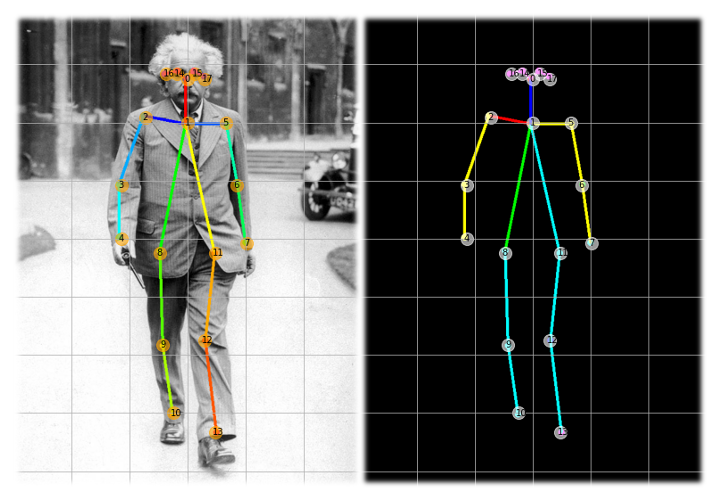
\includegraphics[scale=.5]{Figures/introduction-einstein.png}}
\caption{Example of human pose estimation key points \cite{rovai_realtime_2020}}
\label{example}
\end{figure}

A 3D point cloud is simply a set of points with three positional coordinates and represents points in 3D space. The points represent the shape of the object in 3D space. 3D point clouds are usually gathered by 3D scanners or dual-lens cameras.The output of scanners is point cloud where each point corresponds to some point on scanning surface with predefined precision. With the rapid growth of LIDAR and VR fields, the importance of accurate and fast 3D point cloud human pose estimation algorithms is clear.

\section{Challenges}
The obvious challenge of human pose estimation is the potential space of different human postures. The small change in the body part position changing the target pose. The task gets more complicated with different obstacles like clothes.
Using recent ML algorithms such as deep learning on 3D point cloud results in many challenges. Some of the common issues are:
\begin{itemize}
  \item The high dimensionality of the input space. Compared to pose estimation based on images, 3D point cloud has higher-dimensional space.
  \item Noisy inputs from 3D point cloud scanners. The sparsity and accuracy of the point cloud greatly influence the model's performance. The accuracy and granularity of points are significantly dependent on the scanning device. Compact LIDAR scanning devices the most popular and less accurate.
  \item Geometric-viewpoint relation. The human body has a strict geometric relation between body parts, which is invariant to the viewpoint. Most of the deep learning algorithms are not viewpoint agnostic resulting in additional challenges for human pose estimation.
  \item Lack of data. The amount of data for 3D point cloud human pose estimation is significantly less than regular image datasets. This fact is due to the high complexity of collecting 3D point cloud data, e.g., need special multicamera or LIDAR equipment, need diverse human positions, need different human constitutions.
\end{itemize}

\section{Motivation}
Human pose estimation is an important task that is used in different fields.
A recent class of deep learning architecture known as capsule networks \parencite{sabour_dynamic_2017} theoretically overcomes multiple conventional deep learning models for human pose estimation. Compared to CNNs, capsule networks, due to the dynamic routing algorithm, account for the spatial relation between the input scene parts. Additionally, capsule networks "learn" the object's geometric relationship and thus could be viewpoint agnostic \parencite{sabour_dynamic_2017}. These capsule networks' properties make them the right candidate for examining human pose estimators based on the point cloud.
Moreover, some experiments \parencite{wang_capsule_2020,gritsevskiy_capsule_2018} stated that capsule networks need less data for convergence compared to non-capsule models. Besides, due to latent space inside the capsule network, it is more noise agnostic than regular convolutional networks.

\section{Research Gap}
\begin{itemize}
  \item There is no capsule-based model for 3D human pose estimation task.
  \item There is no comparison of the influence of noisy data on capsule-based and non-capsule-based models for 3D space.
  \item There is no comparison of how well capsule-based works with limited dataset compared to regular models.
\end{itemize}

\section{Objective}
The work's objective is to propose a model based on a capsule network for a 3D point cloud human pose estimation. Evaluate the model on public benchmark dataset for human pose estimation. Compare results with state of the art approaches for the task as mentioned earlier. Evaluate the influence of the noise in training dataset on capsule-based and non-capsule-based networks. Measure the performance of the models with different sizes of training dataset.

\section{Paper structure}
Section \ref{Related work} covers the related work of human pose estimation based on both 2D images and 3D point clouds. This section described conventionally, and state of the art approaches for solving the issue. Reviews capsule networks for different 3D point cloud tasks like point classification, segmentation, and position estimation.

The rest of the paper is organized in the following manner:
\begin{itemize}
  \item Section \ref{Hypothesis} presents the project's hypothesis and problems;
    \item  section \ref{Dataset} describes the dataset which is used for training and evaluation along with evaluation metrics;
  \item  section \ref{Methodology} describes the approach for solving the project's objectives;
   \item  section \ref{Experiments} describes experiments on project's objections described in \ref{Methodology};
  \item  section \ref{Conclusions} sums up the paper's ideas and present brief conclusions and possible future work in this field.
\end{itemize}
\chapter{Related work}
\label{Related work}

In this chapter, we overview common approaches to solve problems with point clouds. We review common techniques, models, and algorithms for point clouds.

In Section~\ref{Deep learning approaches for point cloud} and Section~\ref{Point-based Methods} we review common approaches on how to use point clouds in deep learning, along with preprocessing methods for 3D point data.

In Section~\ref{Human pose estimation} we review models and techniques for the task of human pose estimation, both for 2D and 3D spaces.

In Section~\ref{Capsule network} we review the initial work on the capsule network which were released for the task of image classification. Also, we review few works which adapt capsule networks for 3D point cloud data.

\section{Deep learning approaches for point cloud}
\label{Deep learning approaches for point cloud}
The different number of points and high dimensionality of the point cloud input makes it challenging to use regular 2D convolutions. The typical approach for such an issue is the conversation of the point cloud to a different format. Such approaches are projection-based methods, volumetric-based methods, and other geometric-based methods.
\subsection{Projection-based methods} 
Projection-based methods take point cloud and project it into a different panel view. After the projection, each view provides a set of combined features for target classification, regression, or segmentation. The critical challenge for the projection-based algorithm is the multi-view feature aggregation into one global feature space.

MVCNN \parencite{su_multi-view_2015} is the first CNN-based architecture which recognize rendered views of different shapes independently from each other. The model's performance shows that even from one view the 3D shape could be recognized with competitive accuracy. Adding more views increase the overall accuracy of the model. The processing pipeline if the MVCNN is shown in Figure~\ref{img:mvcnn}.

\begin{figure}[htbp]
    \centerline{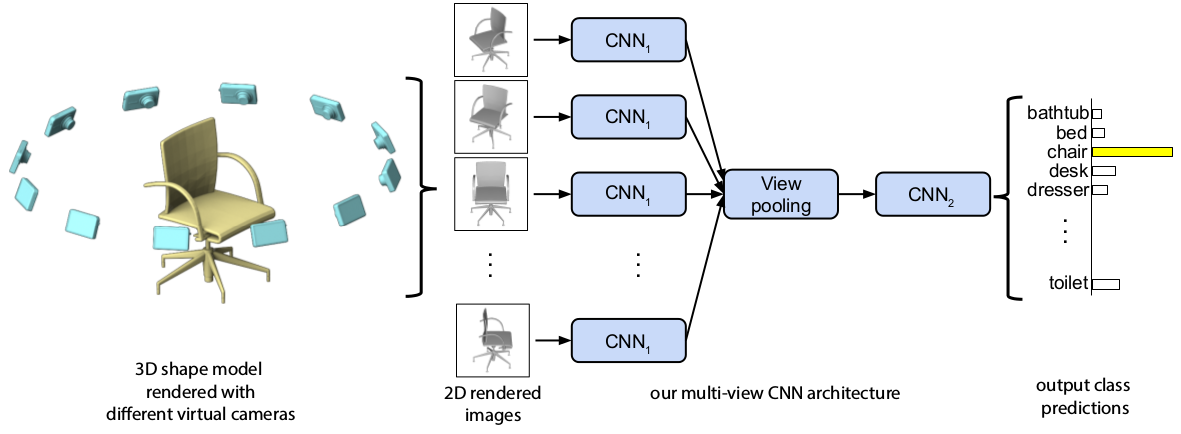
\includegraphics[scale=0.4]{Figures/mvcnn.png}}
    \caption{MVCNN processing pipeline  \parencite{su_multi-view_2015}}
    \label{img:mvcnn}
\end{figure}

MHBN \parencite{yu_multi-view_2018} (Multi-view Harmonized Bilinear Network) is the continuation of MVCNN. The approach proposes to integrates local convolutional features by harmonized bilinear pooling to produce a compact global descriptor.
To persist the information from different views, the View-GCN \parencite{wei_view-gcn_2020} proposes constructing view-graph with multiple views as graph nodes, then designing a graph convolutional neural network over view-graph to learn discriminative shape descriptor hierarchically.
All projection-based methods struggle from high memory consumption and high computational complexity since, for one feature extraction, the model should be run for the number of different views.

\subsection{Volumetric-based methods} 
Volumetric-based methods map the point cloud into a 3D grid. Then conventional 3D convolutions are using for feature extraction.
VoxNet \parencite{maturana_voxnet_2015} is the first method that exploits the volumetric representation of the point cloud. In this work, each cloud point is mapped to a discrete voxel point. The size of the target grid is 32 x 32 x 32 voxels. After the mapping, three convolutional layers are using to produce the target feature representations. Processing steps of VoxNet is shown in Figure~\ref{img:voxnet}

\begin{figure}[htbp]
    \centerline{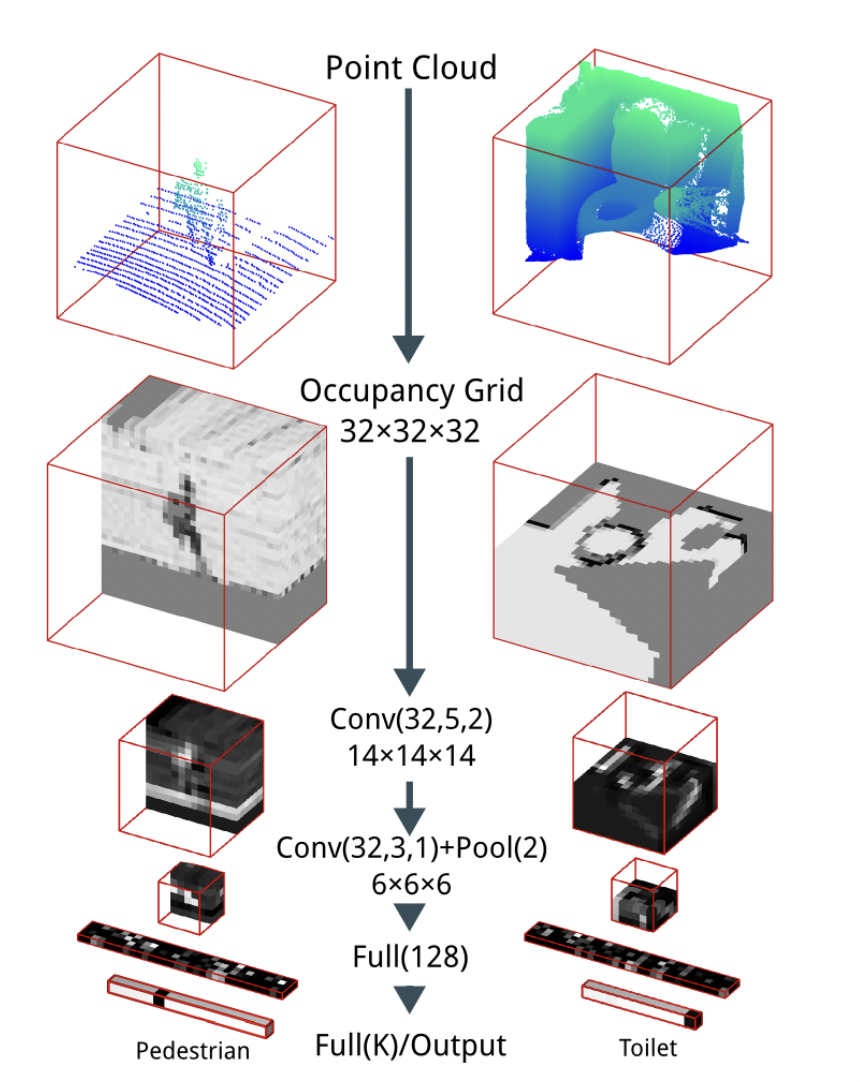
\includegraphics[scale=0.4]{Figures/VoxNet.png}}
    \caption{VoxNet processing pipeline  \parencite{maturana_voxnet_2015}}
    \label{img:voxnet}
\end{figure}

The more advanced volumetric-based models use octrees data structure. OctNet \parencite{riegler_octnet_2017} propose to represent the point cloud as several octrees along a regular grid (Figure~\ref{img:octTree}), each octree is encoded as a bit string, and features are generated through naive arithmetic. This approach reduces the memory consumption of the model during the training and inference stages.
The next iteration of octrees representation of point cloud is proposed in O-CNN \parencite{wang_o-cnn_2017}. The model uses 3D convolutions to extract features from octrees. This model also uses octree representation. The model takes the average normal vectors if 3D model from leafs of octants and runs 3D CNN on this to perform classification.

\begin{figure}[htbp]
    \centerline{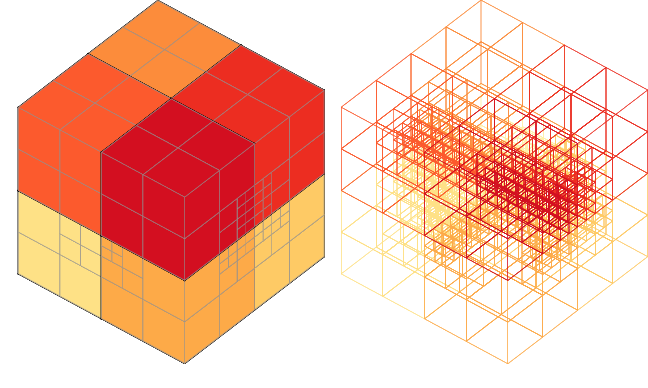
\includegraphics[scale=0.4]{Figures/OctNet.png}}
    \caption{An example of octree grid \parencite{riegler_octnet_2017}}
    \label{img:octTree}
\end{figure}


\section{Point-based Methods}
\label{Point-based Methods}
Compared with projection-based methods and volumetric-based methods that aggregate points from a spatial neighborhood, point-based methods attempt to learn features from individual points. Most of the recent work focuses on this direction.

The first work which uses a point-based approach is PointNet \parencite{qi_pointnet_2017}. PointNet learns pointwise features independently with several MLP layers and extracts global features with a max-pooling layer. The input (an $n \times 3$ 2D tensor) is first multiplied by an affine transformation matrix predicted by a mini-network (T-Net) to hold invariance under geometric transformations. The point set is then passed through a group of MLPs followed by another joint alignment network, and a max-pooling layer to obtain the final global feature. The model's architecture is depict in Figure~\ref{img:pointnet}

\begin{figure}[htbp]
    \centerline{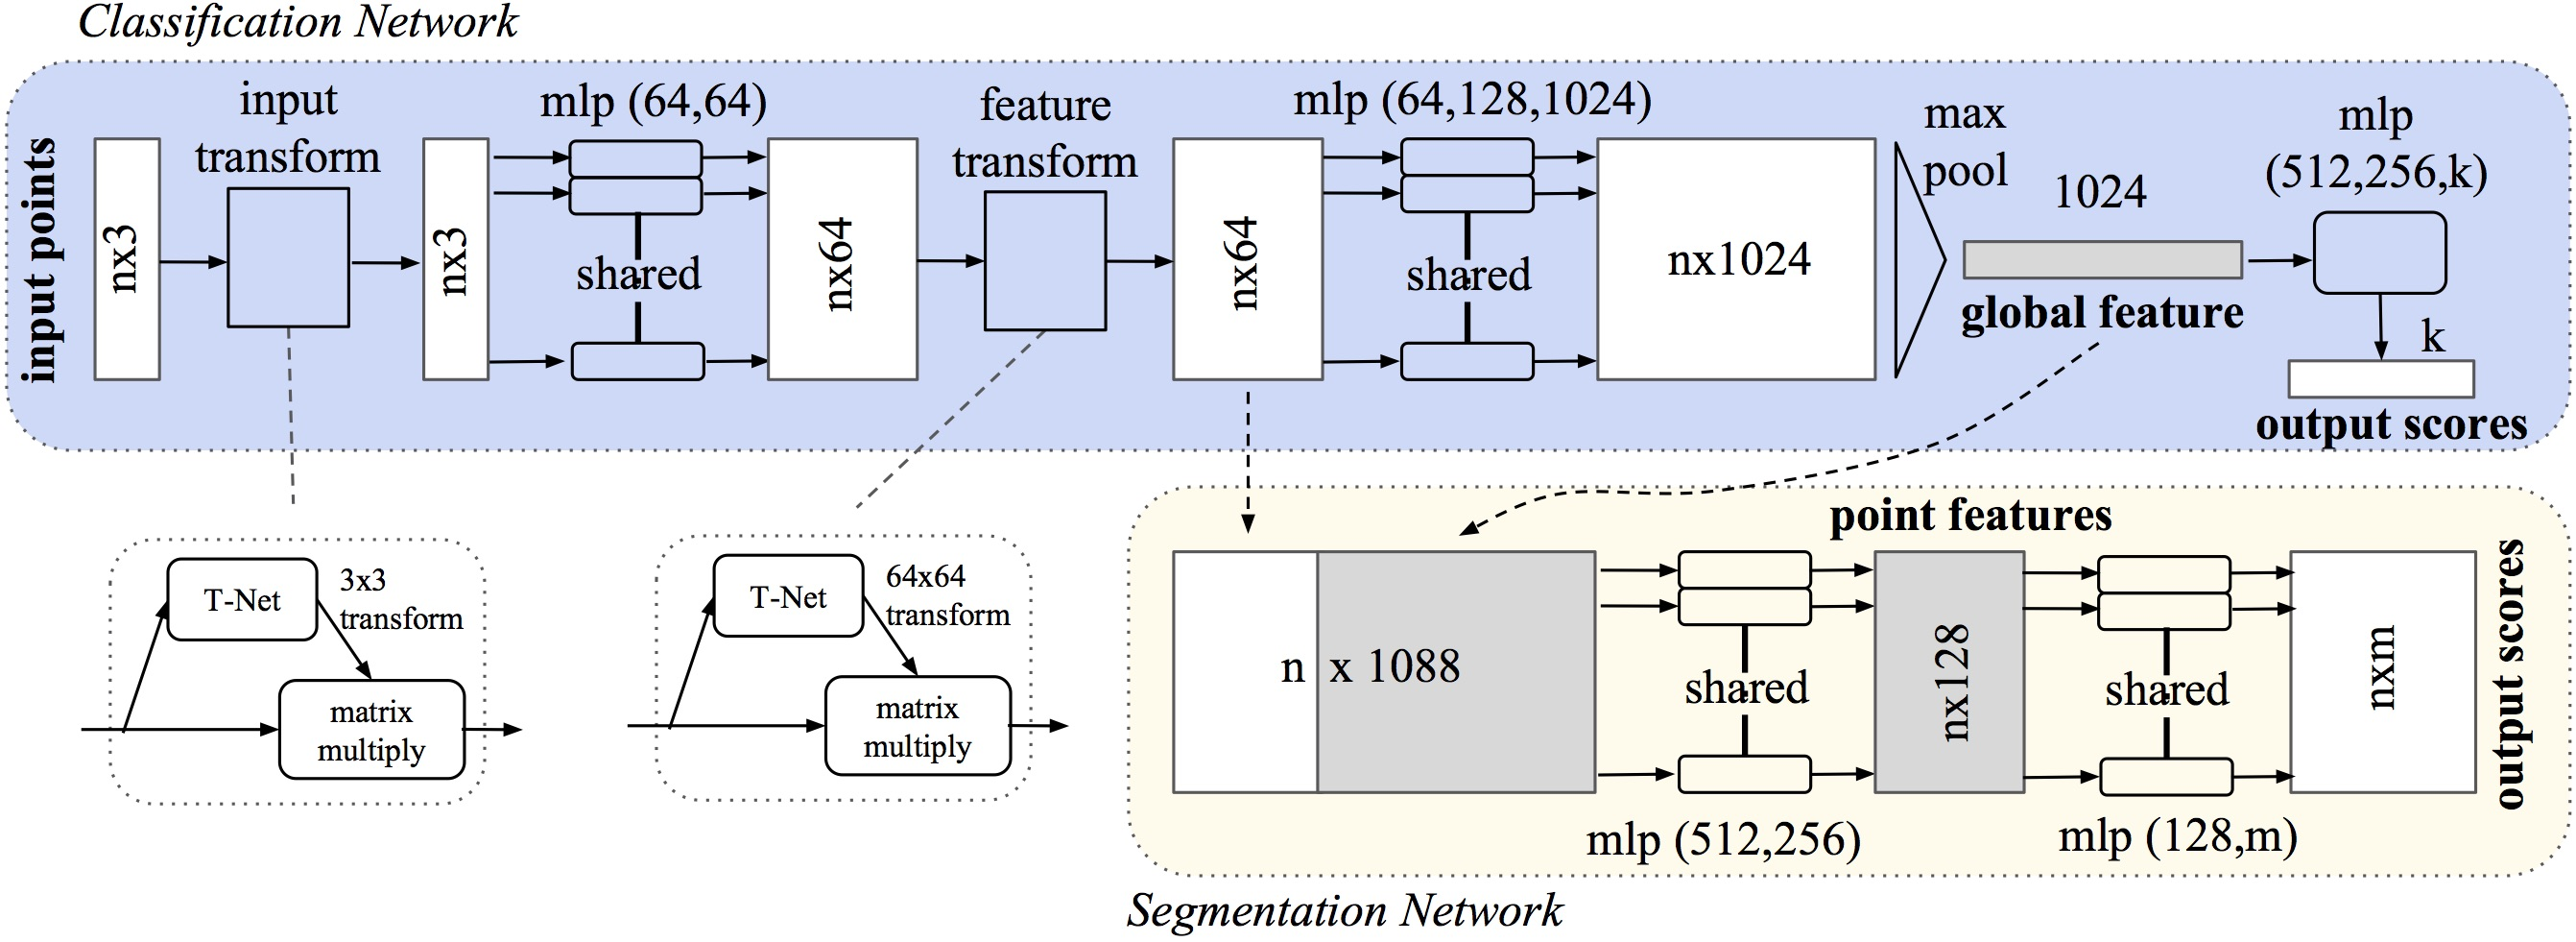
\includegraphics[scale=0.15]{Figures/pointnet.jpeg}}
    \caption{PointNet architecture \parencite{qi_pointnet_2017}}
    \label{img:pointnet}
\end{figure}

The second iteration of PointNet is PointNet++ \parencite{qi_pointnet_2017-1}. PointNet++ introduces a hierarchical neural network that applies PointNet recursively on a nested partitioning of the input point set. Using metric space distance, the model could learn local features with increasing contextual scale.
The state-of-the-art model for point-based classification is Point Attention Transformers \parencite{yang_modeling_2019}. The research for the first time proposes the mechanism of sampling which is end-to-end and task agnostic. The sampling is named "Gumbel Subset Sampling" - GSS. This sampling is used to select the most representative subset of the point cloud from the initial data. Using Gumble-Softmax, the model could provide a continuous point subset in the training phase, and a strict discrete subset in the test phase. Using such an approach the model is able to learn a more robust representation of the input data with less computational complexity.

\section{Human pose estimation}
\label{Human pose estimation}
The latest research approaches in the field of human pose estimation are based on deep learning.
There are two main approaches to the task:
\begin{itemize}
  \item pose estimation based on 2D images (mostly RGB);
  \item pose estimation based on the 3D point cloud.
\end{itemize}

The latter approach is more recent and promising. The 3D perspective gives more information for the models about body position in the space. Also, 3D point clouds mitigate the issue with occluded parts of the body. 2D image is a 2D projection of 3D space, and this transformation leads to the loss of information.

\subsection{Image-based methods}
The approaches for 2D image human pose estimation are divided into two types:
\begin{itemize}
  \item top-down approach
  \item bottom-up approach
\end{itemize}
In the top-down approach, the first step is person detection and then pose regression. In the bottom-up approach, all body parts are detected first and then grouped according to the body's position.

OpenPose \parencite{cao_openpose_2019} is the most popular example of bottom-up approaches for multi-person pose estimation. The network first extracts features from the image using the VGG feature extractor. Then features are passed to two separate branches, the first branch predicts body parts key points, the second branch predicts the associativity between body parts. The result of human pose estimation from OpenPose is shown in Figure~\ref{img:openpose}.

\begin{figure}[htbp]
    \centerline{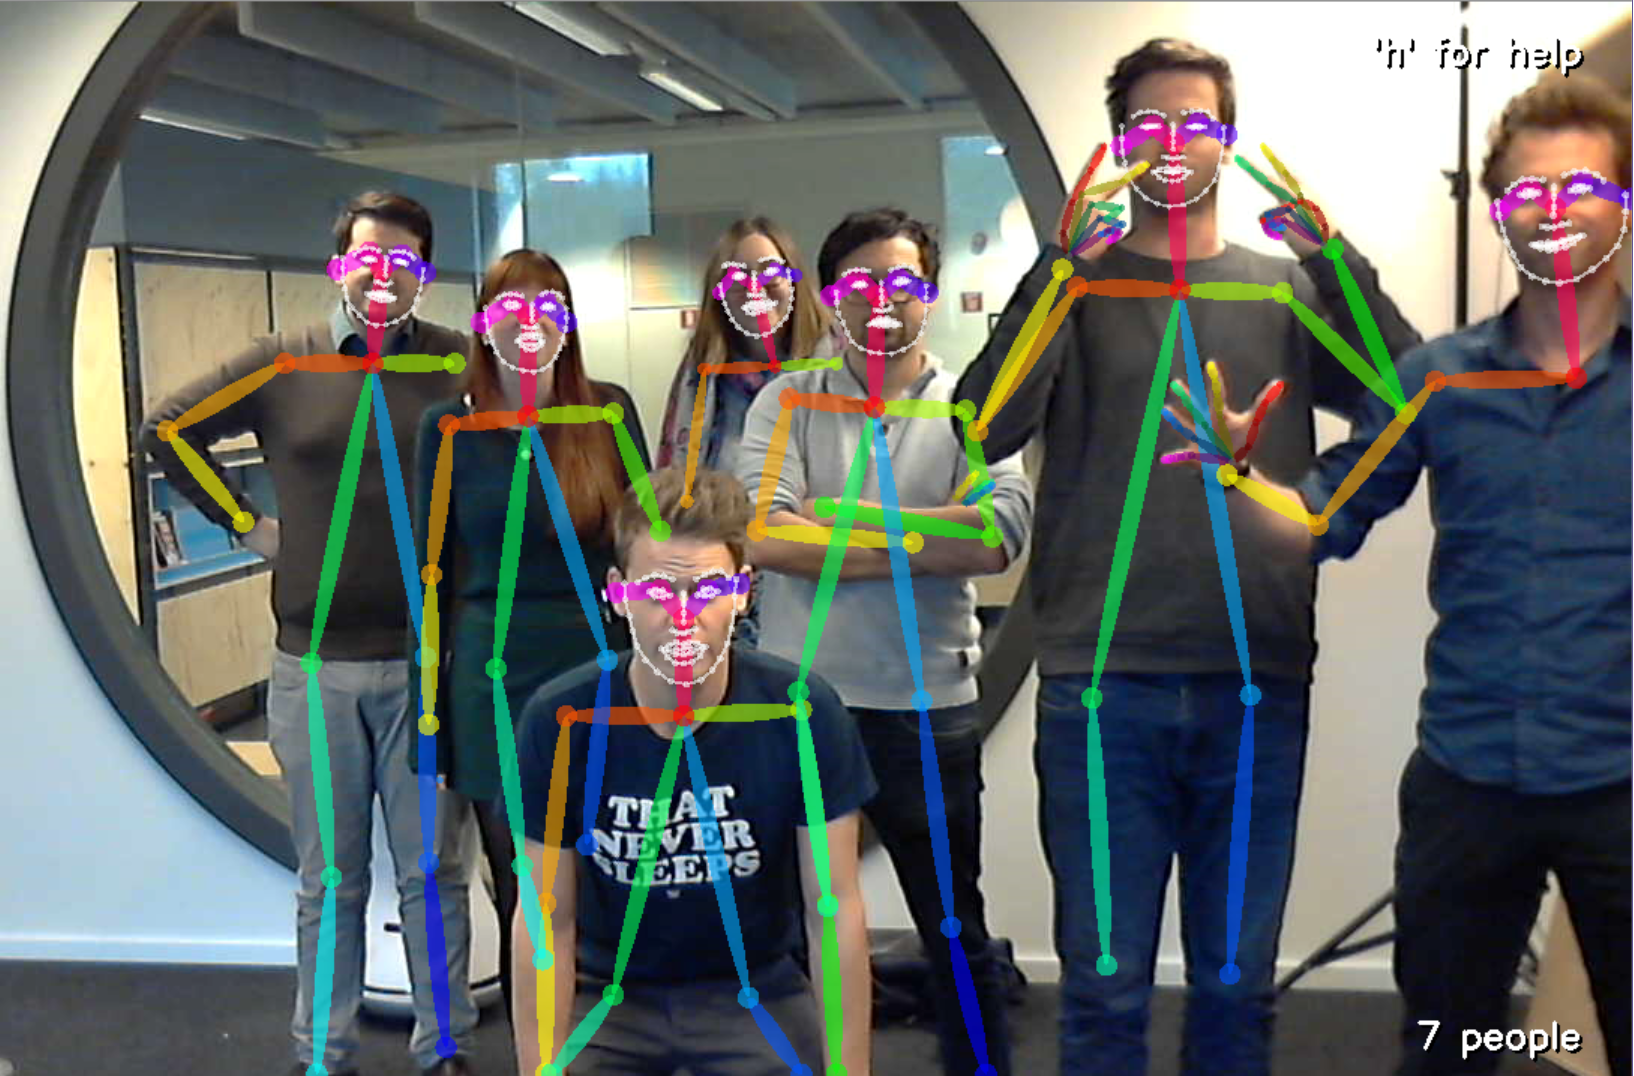
\includegraphics[scale=0.15]{Figures/OpenPose.png}}
    \caption{An example OpenPose network result  \parencite{cao_openpose_2019}}
    \label{img:openpose}
\end{figure}

RMPE (AlphaPose) \parencite{fang_rmpe_2018} is a top-down model.
This approach proposes to use a four-stage pipeline. The first step is Symmetric Spatial Transformer Network (SSTN). In this step, the model extracts the human region using a bounding box. The second step is a Single Person Pose Estimator (SPPE). This step model uses extracted human regions to estimate key joints of the human body. The third step is spatial De-Transformer Network (SDTN). This step remap estimated human joint coordinates back to the original coordinate system. The last step is parametric pose Non-Maximum Suppression (NMS). This step handles the issue with redundant pose deductions.

\subsection{point-cloud-based methods} 
Point cloud-based estimation is a relatively young field due to the recent growth of popularity of point cloud scanning devices.

The first model for human pose estimation based on point cloud was presented by \cite{diaz_barros_real-time_2015}. The paper presents an approach where based on a predefined human body skeleton the input point cloud is clustered using PCA and Expectation maximization algorithms.

The recent work in this field is presented by \cite{zhou_learning_2020}. The work takes point clouds as input data and model the surface of the object, in this research - human body, using deep human pose network. The pros of this approach is that it's an end-to-end model. It takes 2D depth image, transforms it to 3D point cloud, and then estimate key human joint coordinates. The model's architecture is shown in Figure~\ref{img:humreg}

\begin{figure}[htbp]
    \centerline{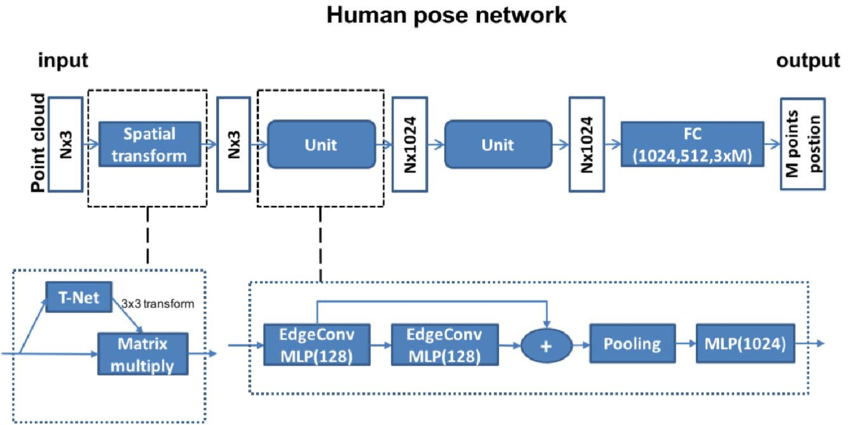
\includegraphics[scale=0.4]{Figures/human-regression-network.png}}
    \caption{Architecture of DNN presented by \parencite{zhou_learning_2020}}
    \label{img:humreg}
\end{figure}

More point cloud human pose estimation methods will be covered in the next subsection. The next subsection covers models which are based on capsule architecture.

\section{Capsule network}
\label{Capsule network}
The concept of the capsule was first proposed by Hinton \parencite{sabour_dynamic_2017} and has been widely used in 2D and 3D deep learning \parencite{kakillioglu_3d_2020, qin_detecting_2020, duarte_videocapsulenet_2018, lalonde_capsules_2018}.

Capsules are represented as a set of vectors. The length of the capsule's vector represents the probability of the object's presence. The direction of the vector describes the object's property e.g. position, viewpoint, size, shape, etc. For capsules' training Hinton proposes a new algorithm \parencite{sabour_dynamic_2017} called dynamic routing. The forward pass with dynamic routing propagates the input data from lower-level capsules to higher-level ones. Lower-level capsules pass learned and predicted data to the higher-level capsules. If multiple lower-level capsules agree (activated) then higher-level capsules activate accordingly. With each iteration of dynamic routing, each capsule gets more accurate.

\subsection{Capsule networks for point cloud classification}
The first work where capsule networks were applied to the problem of point cloud classification is 3DCapsNet \parencite{cheraghian_3dcapsule_2018}. In this work, a new capsule-based layer is proposed - ComposeCaps. ComposeCaps learns spatially relevant feature mapping that can be exploited for 3D point cloud classification. The architecture of the network is shown in Figure~\ref{img:3DCapsNet}

\begin{figure}[htbp]
    \centerline{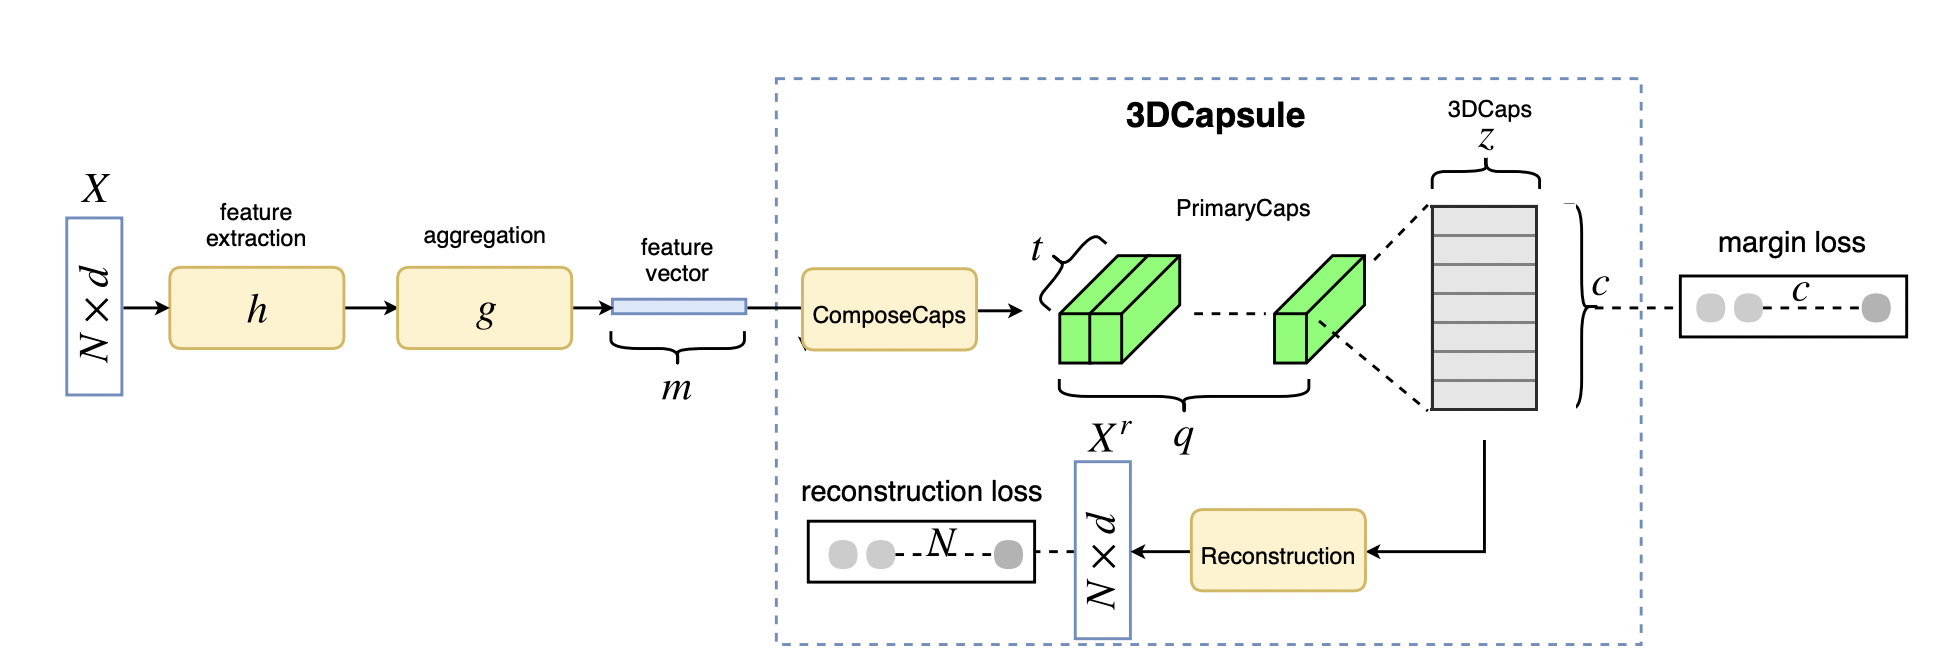
\includegraphics[scale=0.4]{Figures/3DCapsNet.png}}
    \caption{The architecture of 3DCapsNet \parencite{cheraghian_3dcapsule_2018}}
    \label{img:3DCapsNet}
\end{figure}

The second iteration of capsule applicability to 3D classification is the 3D point capsule network \parencite{zhao_3d_2019}. 3D point capsule network is an auto-encoder designed based on capsule networks. In this work researchers propose new architecture with a capsule network encoder that encodes input point cloud to capsules' latent space, and a decoder that decodes latent capsules. The proposed architecture works for several common point cloud-related tasks, such as object classification, object reconstruction, and part segmentation.

\subsection{Capsule networks for point cloud regression} 
The only work which is currently presented on the topic of point cloud regression is Capsule-HandsNet \parencite{wu_3d_2020}. This project is inspired by this research. Capsule-HandsNet uses model based on capsule auto-encoder proposed in \cite{zhao_3d_2019}. The model is an end-to-end, it takes hand point cloud and predicts key joints. The latent space of the model provides an ability to "memorize" the internal structures of the object such as symmetry, junction, relative location of object's parts, etc. The restored point cloud is combined from local patches predicted by capsules inside of the decoder (Figure~\ref{img:capshandnet}).   

\begin{figure}[htbp]
    \centerline{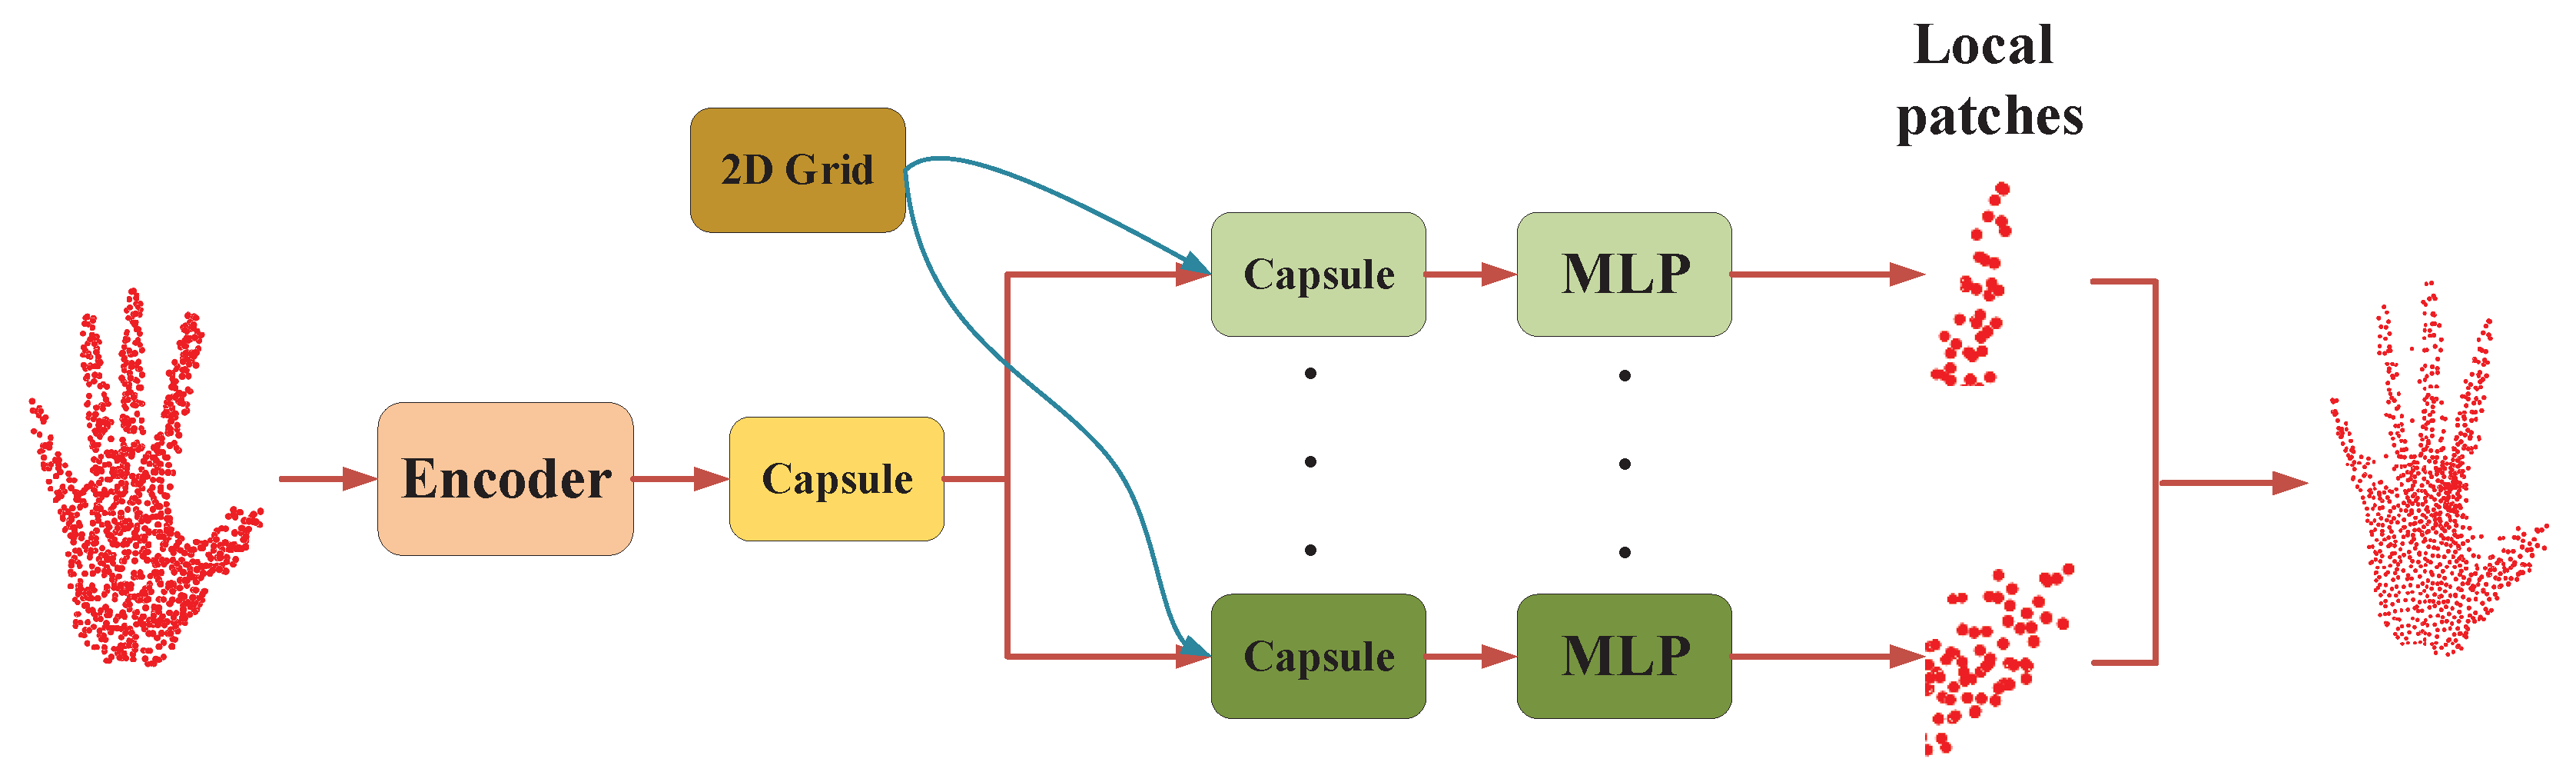
\includegraphics[scale=0.9]{Figures/caps-hand-net.png}}
    \caption{Reconstructed point cloud from capsule local patches \parencite{wu_3d_2020}}
    \label{img:capshandnet}
\end{figure}
 
\chapter{Research Hypothesis and Problem}

\label{Hypothesis}

\section{Hypotheses}
\paragraph{Model Comparison hypothesis:} This project's main objective is to create a model for human pose estimation based on point cloud using a capsule-based neural network, which shows competitive accuracy on well-known benchmarks.

\paragraph{Noise resistance hypothesis:} the impact of noise in the training dataset on the capsule-based model should be less compared to non-capsule models. Hypothesis is made based on 2D image recognition based using capsule networks \cite{sabour_dynamic_2017}.
Dataset size hypothesis: The dataset's size for full convergence should be smaller for capsule-based network compared to non-capsule ones. Assumption is made based on experiments presented in \cite{sabour_dynamic_2017} based on 2D image classification.

\section{Problems}
\paragraph{Noise problem.} To achieve the project goal mentioned above, we need to create an algorithm that could create realistic noise for point cloud data. We need to analyze and replicate factors that influence scanning devices' accuracy and result in noisy data.
\paragraph{Models' retrain problem.} To achieve the project's third goal, we need to retrain reference sota models with truncated training data. Hence, we need to allocate additional time for such an activity.
%\include{Chapters/Chapter4} 
%\include{Chapters/Chapter5} 

%----------------------------------------------------------------------------------------
%	THESIS CONTENT - APPENDICES
%----------------------------------------------------------------------------------------

\appendix % Cue to tell LaTeX that the following "chapters" are Appendices

% Include the appendices of the thesis as separate files from the Appendices folder
% Uncomment the lines as you write the Appendices

% Appendix A

\chapter{Frequently Asked Questions} % Main appendix title

\label{AppendixA} % For referencing this appendix elsewhere, use \ref{AppendixA}

\section{How do I change the colors of links?}

The color of links can be changed to your liking using:

{\small\verb!\hypersetup{urlcolor=red}!}, or

{\small\verb!\hypersetup{citecolor=green}!}, or

{\small\verb!\hypersetup{allcolor=blue}!}.

\noindent If you want to completely hide the links, you can use:

{\small\verb!\hypersetup{allcolors=.}!}, or even better: 

{\small\verb!\hypersetup{hidelinks}!}.

\noindent If you want to have obvious links in the PDF but not the printed text, use:

{\small\verb!\hypersetup{colorlinks=false}!}.

%\include{Appendices/AppendixB}
%\include{Appendices/AppendixC}

%----------------------------------------------------------------------------------------
%	BIBLIOGRAPHY
%----------------------------------------------------------------------------------------

\printbibliography[heading=bibintoc]

%----------------------------------------------------------------------------------------

\end{document}  
